\documentclass{scrartcl}
\usepackage[utf8]{inputenc}
\usepackage[T1]{fontenc}
\usepackage[ngerman]{babel}
\usepackage{amsmath}
\usepackage{graphicx}
 
\title{Praktikum Betriebssysteme: Projekt 1\\ Client/Server Stream Socket Programmierung}
\author{Andreas Ruscheinski\thanks{Matr.-nr.: 211203494}\and Christian Delfs\thanks{Matr.-nr.: 211204103}\and Fabienne Lambusch\thanks{Matr.-nr.: ?????????}}
\begin{document}
\maketitle
\tableofcontents

\section{Problem}
	Ziel des Projektes war es, zu lernen, wie Dateien mit Hilfe von Client/Server Stream Socket Programmierung (mit TCP/IP Sockets) angelegt und verwaltet werden können. Das wie folgt beschriebene Grundsystem wurde von uns mit einem Datei-Zugriffsschutz erweitert. 
	Unsere Gruppe hat sich für Option b) entschieden: den Datei-Zugriffsschutz. Hierbei wird zwischen normalen Nutzern und Administratoren unterschieden, die sich durch verschiedene Rechte auszeichnen. Nach einem Login, der zum einen die Gültigkeit prüft, werden an dieser Stelle auch die Rechte ermittelt. Durch die Rechteverteilung werden dem Nutzer auf Clientseite verschiedene Funktionen zur Auswahl gestellt.\\

\section{Vorbetrachtung - Theorie}
	\subsection{Grundfunktionalitäten}
		Die grundlegenden Anforderungen an das Softwarprojekt sind wie folgt gegeben:
		\begin{enumerate}
		\item Speicherung der Studenten in separate Datensätze auf der Server-Seite. Enthaltene Informationen: Name, Matrikel-Nr., Geburtsdatum, Noten von n
		Lehrveranstaltungen.
		\item Es gibt m Gruppen von Studenten, die jeweils mehrere Studenten umfassen (m >= 3).
		\item Jede Gruppe repräsentiert einen Studiengang.
		\item Die Datensätze jeder Gruppe werden in einer eigenen Datei gespeichert.
		\item Gruppenbesten anhand des Durchschnitts ermitteln.
		\item Mindestanforderungen: Mindestens drei Gruppen und in jeder: mindestens drei Studenten und jeder Studentendatei: mindestens drei Noten
		\item Die Datensätze der Studenten sollten zugreifbar sein.
		\item Bester aller Studenten soll ermittelbar sein.
		
		\end{enumerate}
	\subsection{Kommunikation zwischen Server und Client}
		Für unser Projekt verwenden wir verbindungsorientierte Sockets. Es wird eine festbestehende Verbindung zwischen dem Client und Server aufgebaut. Mit diesem Hilfsmittel wird ein Datenaustausch ermöglicht, der erlaubt, dass Daten zwischeneinander versendet werden können.\\
		Der theorethische Ablauf, wie die Kommunikation erfolgt ist wie folgt:
		\textbf{Client-seitig:}
		\begin{enumerate}
			\item Socket erstellen
			\item erstellten Socket mit der Server-Adresse verbinden, von welcher Daten angefordert werden sollen
			\item senden und empfangen von Daten
			\item evtl. Socket herunterfahren (shutdown())
			\item Verbindung trennen, Socket schließen
		\end{enumerate}
		
		\textbf{Server-seitig:}
		\begin{enumerate}
			\item Server-Socket erstellen
			\item binden des Sockets an eine Adresse (Port), über welche Anfragen akzeptiert werden
			\item auf Anfragen warten
			\item Anfrage akzeptieren und damit ein neues Socket-Paar für diesen Client erstellen
			\item bearbeiten der Client-Anfrage auf dem neuen Client-Socket
			\item Client-Socket wieder schließen
		\end{enumerate}

	\subsection{Dateizugriff}
		In unserm Projekt nutzen wir das CDV-Dateiformat um die Datensätze von Studenten auf eine praktische Art und Weise speichern und auslesen zu können. Um die Studenten ihrer zugehörigen Gruppen zuzuordnen, werden diese in Verzeichnissen abgelegt.\\
		Diese Verzeichnisse werden anhand ihrer Bennenungen unterschieden, z.B.: steht der Ordner ITTI für die Studenten, die der Informationstechnik / Technische Informatik angehören.\\
		Generell werden Studenten in einer Datei gespeichert, die als Bezeichnung die zughörige Matrikelnummer besitzt. Innerhalb der Datei befinden sich die folgenden Datensätze, durch Simikolons von einander getrennt:\\
		\begin{itemize}
			\item Passwort
			\item Vorname
			\item Nachname
			\item Matrikelnummer
			\item zugehöriger Studiengang
			\item Geburtstag
			\item eine beliebiege Anzahl an Noten
		\end{itemize}
		Der Datensatz eines Beispielstudenten sieht folgender Maßen aus:\\
		 \\
		mukitkarP;Max;Mustermann;113116119;Informatik;23.05.2013;1.0;1.3;2.7;5.0;1.0\\
		 \\
		Innerhalb des Programmes werden, bis auf die Noten, die Datensätze als Char-Arrays gespeichert. Wichtig ist es darauf zu achten, dass an letzter Stelle das Terminationszeichen ist. Das Passwort darf aus maximal 10 Zeichen bestehen. Für Vorname, Nachname und der zugehörige Studiengang sind 20+1 Char zur Verwendung unterstützt. Die Matrikelnummer besitzt 9 Stellen. Diese wird folglich in 9+1 Chars vom Client abgefragt. Ähnlich bei dem Geburtstag der in der Form DD.MM.YYYY in 11 Chars gespeichert wird. \\
		Sowohl die einzelnen Noten, als auch die berechneten Durschnitte sind vom Datentyp Double. In die Datei werden die Noten als Chars der Länge 4 eingetragen, sodass sie immer die folgende Form besitzen X.Y wobei 1<X<5 und Y$\in \{$0,3,7$\}$ ist.\\
		\subsubsection{Beipieldatein}
			Da zu Laufzeiten des Programms sowohl Gruppen als auch Studenten mit einer beliebigen Anzahl an Noten hinzugefügt werden, decken unsere Beispieldatein den geforderten Teil ab:
			
			\textbf{Gruppen:}
			\begin{itemize}
				\item Informatik
				\item ITTI
				\item Elektrotechnik
			\end{itemize}
			
			\textbf{Studenten der Informatik:}
			\begin{itemize}
				\item 123;Tom;Klein;100000010;Informatik;01.01.19901.0;4.0;1.7;3.0
				\item 234;Max;Mustermann;100000011;Informatik;23.05.2001;1.0;1.3;2.7
				\item 345;Benjamin;Groß;100000012;Informatik;14.12.1986;1.0;1.3;2.7;3.3;1.7;5.0
			\end{itemize}
			
			\textbf{Studenten der ITTI:}
			\begin{itemize}
				\item 456;Even;Longer;100000013;ITTI;15.11.1977;1.3;2.7;3.3;1.7;5.0;1.0
				\item 567;Very;Long;100000014;ITTI;12.05.1993;1.0;1.3;2.7;1.0;5.0;1.0;1.0;1.0
				\item 678;Alfons;Hatler;100000015;ITTI;14.03.1989;1.0;1.0;1.0;1.0
			\end{itemize}
			
			\textbf{Studenten der Elektrotechnik:}
			\begin{itemize}
				\item 789;John;McClane;100000016;Elektrotechnik;24.12.1966;1.3;3.7;5.0;4.0
				\item 890;Hans;Gruber;100000017;Elektrotechnik;15.07.1991;1.3;5.0;2.7;1.0;4.0;1.7;3.0;2.0
				\item 901;Holly;McClane;100000018;Elektrotechnik;30.08.1988;1.7;1.3;1.3;1.7;1.0;1.7;1.7
			\end{itemize}
		
	\subsection{Umzusetztende Funktionalitäten}
		Neben den geforderten Funktionen, haben wir unser Programm um einige ausgewählte Funktionen bereichert. Unter Berücksichtigung der zwei Zugriffsarten mit unterschiedlichen Rechten werden hier die Funktionalitäten an zugehöriger Stelle beschrieben.\\
		Dem Nutzer werden diese Möglichkeiten nach dem Login in einer Menüform zur Auswahl gestellt. Die Auswahl eines Menüpunktes erfragt auf Client-Seite, wenn nötig, Eingaben bzw. gibt die gewünschten Ergebnisse zurück.
		\subsubsection{Administrator}
			\begin{description}
				\item[Studenten anlegen] Der Administrator muss bei dem Erstellen eines neuen Studenten dessen Vorname, Nachname, Matrikelnummer, Studiengang und Geburtstag angeben. Durch diese Eingabe wird eine Datei mit der Matrikelnummer als Name und im passenden Ordner (dem Studiengang) angelegt.
				\item[Gruppe anlegen] Durch diese Funktion wird ein neues Verzeichnis erstellt, in das später Studenten eingefügt werden können.
				\item[Studentendaten anzeigen] Um die Daten eines Studenten einzusehen, werden Kentniss über seinen Studiengang und sine Matrikelnummer vorrausgesetzt. Zusätzlich wird auch dessen Durschnitt angezeigt.
				\item[Guppe anzeigen] Nach der Eingabe des Studiengangs als Gruppennamen, werden alle Studenten aus diesem ausgegeben.
				\item[Note hinzufügen] Damit einem Studenten eine Note hinzugefügt werden kann müssen Studiengang, Matrikelnummer und die hinzuzufügende Note als Eingabe angegeben werden.
				\item[Gruppenbesten ermitteln] Für die ausgewählte Gruppe wird der beste Student anhand der einzelnen Durchschnitte ermittelt.
				\item[Gesamtbesten ermitteln] Von allen Studenten, die gespeichert sind, wird der, mit dem besten Durchschnitt, ausgegeben.
				\item[Beenden] Beendet die Kommunikation mit dem Server und schließt das Programm auf Seite des Clients.
			\end{description}
			\subsubsection{Normale Nutzer}
			\begin{description}
				\item[Daten anzeigen] Neben dem  Vornamen, Nachnamen, Studiengang, Geburtstag und der Matrikelnummer wird der Durchschnitt ausgegeben.
				\item[Beenden] Beendet die Kommunikation mit dem Server und schließt das Programm auf Seite des Clients.
			\end{description}
\section{Praktische Umsetzung}
	\subsection{Menü}
		Die in Kapitel 2.4 Beschriebenen Funktionalitäten führen zu zwei unterschiedlichen Menü-Formen. Abhängig von den Rechten, die dem Nutzer nach dem Login zugeteilt werden, wird ein entsprechendes Menü angezeigt. 
		\begin{center}
		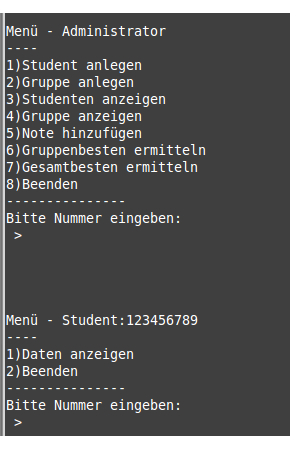
\includegraphics[scale=0.6]{menue.jpg}
		\end{center}
	\subsection{Client}
		Der Client bietet dem Nutzer die Möglichkeit anhand eines Menüs Funktionen auszuwählen. Bei Auswahl werden gegebenenfalls Daten vom Nutzer angefordert und eine Mitteilung über das Ergebnis gegeben. Die Eingaben des Nutzers werden bis zu einem gewissen Grad validiert. Beispielsweise wird verhindert, dass bei der Eingabe Simikolons versendet werden können, da zusätzliche in CSV-Datein und deren Auswertung zu Fehlern führen werden.\\
		In unserem Programm ist es die Hauptaufgabe des Clients eine Schnittstelle zwischen Nutzer und Server darzustellen.
	\subsection{Server}
		Die Aufgabe des Servers ist es, auf die Befehle des Clients zu reagieren. Der Client sendet hierfür die Nummer der Option, die der Nutzer ausgewählt hat. Der Server empfängt diese und reagiert dem entsprechend. Eine große Rolle spielt der Dateizugriff auf Server Seite, da dieser hauptsächlich Dateien schreibt oder ausliest. Anschließend werden die Informationen aufbereitet und an den Client übermittelt. Wie in unserem Projekt dieser Umgang mit Dateien ermöglicht wird, ist wie folgt:
		\subsubsection{Dateien auslesen}
			Da Studiengänge durch Verzeichnisse umgestezt werden, ist es elementar notwendig diese Ordner zu öffnen, um Zugriff auf eine spezielle Studentendatei zu erhalten. Danach wird die Datei vollständig ausgelesen und innerhalb des Programmes zur weiteren Bearbeitung hinterlegt. Die Daten über den Studenten befinden sich jetzt in einem String gespeichert, wobei die Datensätze durch Simikolons getrennt sind. Es ist nun nötig den String aufzugliedern und die benötigten Daten zu extrahieren. Die ermittelten Daten stehen daraufhin zur weiteren Verarbeitung zur Verfügung.
			\begin{description}
				\item[Verzeichnissinhaltsausgabe] wird durch die Funktion opendir() ermöglicht. Der Server erhält den Namen des Verzeichnisses, das geöffnet werden soll und nutzt dafür opendir(). Als Rückgabe erhalten wir einen Pointer, der auf den ersten Eintrag zeigt. Bestimmte Datein, die keine Studenten repräsentieren werden ignoriert. Alle anderen werden nacheinander ausgegeben. Realisiert wird dies in der Funktion findGroup(). An den Server werden die Studenten übermittelt und dort ausgegeben.
				\item[Verzeichnisse öffnen] ist durch chdir() möglich. Der Client übermittelt dem Server welches Verzeichnis geöffnet werden soll. Sollte das öffnen nicht möglich sein, wird dies dem Client umgehend mitgeteilt, die Funktion wird beendet und der Client bekommt die Möglichkeit im Hauptmenü einen neuen Vorgang zu starten. Ist es jedoch möglich gewesen in ein Verzeichnis zu wechseln, kann nun auf alle Dateien innerhalb dieses zugegriffen werden. Wichtig ist, dass im Anschluss daran wieder in das darüberliegende Verzeichniss zurück gewechselt wird. Andernfalls kann es zu Fehlern kommen, da entsprechende andere Studiengänge sich nicht in dem vorher ausgewählten befinden.
				\item[Dateien auslesen] wird durch fscanf(Quelle,Formatierung,Ziel) umgesetzt.
				\item[String aufteilen] realiseren wir mit  strtok(Quellstring, delimiters);. Mit strtok kann ein String anhand von Trennzeichen zerteilt und die einzelnen Abschnitte herausgelesen werden. Die Trennzeichen werden im Parameter delimiter (Begrenzungszeichen, Separator) übergeben - in unserem Fall das Simikolon. Die einzelnen Datensegmente werden in einen anderen String gespeichert, der in Abschnitte unterteilt ist. \\
				\textbf{FABIENNE HIER BITTE NOCHMAL GRÜNDLICH NACHLESEN!!!}
			\end{description}
		\subsubsection{Dateien schreiben}	
			Das schreiben und damit das Anlegen neuer Dateien spielt beim Hinzufügen neuer Studenten bzw. dem Hinzufügen einzelner Noten eine Rolle. Um einen Studenten zu erstellen, muss der ausgewählte Studiengang als aktuelles Verzeichniss gewählt werden. Wenn ein neuer Student angelegt werden soll, werden zuerst noch verschiedene Fehlerfehle abgefangen: Beispielsweise falsches Verzeichnis, Fehler bei Vergabe der Matrikelnummer, etc. \\
			Kam es zu keinen Fehlern wird mit fopen() eine Datei erstellt. Durch fprintf(NeueDatei,Formatierungsstring, MatrikelNummer,Daten) wird in Datei geschrieben. Abschließend wird die Datei geschlossen und wieder in das nächst höhere Verzeichniss zurückgewechselt.
		\subsubsection{Sonstige Funktionen}
			Bisher nicht genauer spezifizierte Funktionen werden mit den gleichen Methoden, wie vorangehend beschrieben, umgesetzt. Ziel und Zweck dieser Funtkionalitäten sind im Nutzerhandbuch beschrieben.
\section{Nutzerhandbuch}
	\subsection{Inbetriebnahme}
		Als Betriebssystem wird eine Linux Distribution vorrausgesetzt. Um das C Programm zu kompilieren, führt der Nutzer im Terminal $\glqq$make install$\grqq$ aus. Wichtig ist, dass er sich im richtigen Verzeichnis befindet - in dem sich auch das Skrip $\glqq$makefile$\grqq$ befindet. In zwei verschiedenen Terminals werden nun die ausführbaren Datein gestartet.\\
		In Terminal 1 wird durch $\glqq$./servern$\grqq$ der Server gestartet.\\
		Den Client startet der Nutzer in dem Terminal 2, durch die Eingabe von $\glqq$./clientn 127.0.0.1$\grqq$.
	\subsection{Server}
		Auf Seiten der Servers werden keine Eigaben oder Interaktionen zur Verfügung gestellt. Es werden gegebenenfalls Rückmeldungen ausgegeben, wenn der Client mit dem Server interagiert. Die Dateipflege kann neben dem Client-Interface auch manuell gehandhabt werden: Ordner als Studiengang hinzufügen, neue Dateien als Studenten anlegen oder Dateien öffnen und bearbeiten. Bei Einhaltung der oben genannten Spezifikationen kommt es dadurch zu keinen Fehlern.
	\subsection{Client}
		Bei Nutzung des Clients im Terminal 2 führt das Programm den Nutzer durch eine intutive Menüführung. Zurück zu dem Hauptmenü kann der Nutzer jeder Zeit durch die Eingabe einer 0 gelangen.
		\subsubsection{Login}
			Nach Starten des Servers werden der Nutzername und das zugehörige Passwort abgefragt. Authentifizieren tuen sich die Studenten durch ihre Matrikelnummer und das zugehörige Passwort. 
			Die Administratoren besitzten den Nutzernamen $\glqq$Admin$\grqq$ und das Passwort $\glqq$abcd$\grqq$.
		\subsubsection{Studenten anlegen}
			Einen neuen Studen anlegen ist nur für Administratoren möglich. Dieser wird aufgefordert stückchenweise dei Stammdaten des Studenten einzugeben: Vorname, Nachname, Matrikelnummer, Studiengang und Geburtstag.\\
			Hierbei wird der Ersteller auf die maximale Länge der Eingabe hingewiesen. Nachdem alle Daten eingeben wurden müssen die Daten noch mit einer $\glqq$1$\grqq$ bestätigt werden. Hiernach wird durch diese Eingabe  eine Datei mit der Matrikelnummer als Name und im passenden Ordner (dem Studiengang) angelegt.
		\subsubsection{Gruppe anlegen}
			Hier wird dem Administrator die Möglichkeit gegeben, bei Bedarf, einen neuen Studiengang hinzuzufügen. Auch hier wird ein Name mit der maximalen Länge von 20 Zeichen angefordert, sodass, nach der Bestätigung, ein neues Verzeichnis mit diesem Namen erstellt wird.
		\subsubsection{(Studenten)daten anzeigen}
			Je nachdem wer diese Funktion aufruft ereignen sich unterschiedliche Interaktionen. \\
			Wenn jemand mit Administrator-Rechten sich Studentendaten anzeigen lassen möchte, wird er gefragt welchem Studiengang der Student angehört und welche Matrikelnummer dieser besitzt.\\
			Handelt es sich um einen Studenten, ist keine Angabe seiner Matrikelnummer nötig. Es werden gleich seine Daten ausgegeben.\\
			In beiden Fällen werden alle Daten und der zugehörige, bei Anfrage berechnete, Durchschnitt ausgegeben.
		\subsubsection{Gruppe anzeigen}
			Diese Funktion ist für Administratoren dahin gehend interessant, da sie für eine Gruppe alle Studenten ausgiebt, die sich in ihr befinden. Dazu ist es nötig den Namen des Studiengangs anzugeben.
		\subsubsection{Note hinzufügen}
			Für ein Software-Projekt, wie dieses, ist es sinnvoll, dass Studenten weitere Noten hinzugefügt werden können. Damit nicht jeder Student sich selbst Noten geben kann, ist dies nur vom Administrator aus möglich. Hierfür müssen wieder Studiengang und Matrikelnummer des Studenten angegeben werden. Dazu kommt naheliegender Weise auch die Note die dem Studenten zugedacht ist. Nach einer Bestätigung wird nun in der Studentendatei hinten die Note angefügt.
		\subsubsection{Gruppenbesten ermitteln}
			Diese Funktionalität ist ebenfalls den Administratoren vorbehalten. Es wird aus jedem Studiengang der Beste ermittelt. Dafür werden von allen Studenten die Durchschnitte gebildet und miteinander verglichen. Studenten wird nicht die Möglichkeit gegeben ihren Durchschnitt mit anderen zu vergleich. Diese Funktion bleibt Administratoren vorbehalten.
		\subsubsection{Gesamtbesten ermitteln}
			Ähnlich wie bei dem Gruppenbesten werden auch hier Studenten verglichen. Um den Gesamtbesten zu ermitteln werden die Gruppenbesten anhand ihrer Durchschnitte verglichen. Nur Administratoren können den Besten ermitteln.
		\subsubsection{Beenden}
			Beendet die Kommunikation zwischen Client und Server. 
\end{document}